\chapter{Методы и протоколы обмена информацией в режиме реального времени, доступные в веб-платформе}

\section{Концепция веб-приложений, работающих в режиме реального времени}

Коммуникация в режиме реального времени (Real-time communication) — вид коммуникации, в котором субъекты могут обмениваться информацией мгновенно или с незначительными задержками передачи \cite{RealTimeCommunicationBase}.

Приложение работающие в режиме реального времени (Real-time application) — это приложения, функционирующие в пределах временных рамок, которые пользователь воспринимает как текущие. Зачастую, приложения, работающие в режиме реального времени, используют событийную архитектуру, для асинхронной обработки поступающих данных \cite{RealTimeCommunicationBaseTwo}.

Обычно, системы реального времени делят на две основные категории: жесткие и мягкие \cite{IntroRealTimeEthrenet}.

\begin{enumerate} 
  \item Жесткие системы реального времени — системы, в которых неправильная работа может привести к катастрофическим событиям. К данной категории относятся различные медицинские системы, системы управления полетами или железнодорожным транспортом.
  
  \item Мягкие системы реального времени — системы, в которых ошибки возникшие в работе системы не приведут к катастрофически последствиям. Примерами таких систем являются системы обмена сообщениями или онлайн-бронирования, где даже небольшие задержки вызовут неудобства у пользователей.
\end{enumerate}

\section{Использование цикличных HTTP запросов для обновления состояния приложения}

Изначально, все веб-сайты разрабатывались на основе модели запрос/ответ, где клиент всегда является инициатором транзакций, запрашивая данные с сервера. Таким образом, у сервера отсутствовал механизм отправки информации без предварительного запроса от клиента.

Создание веб-приложений, где требуется двунаправленная связь между клиентом и сервером, требовало злоупотреблением HTTP для опроса сервера на наличие обновлений. Для обновления состояния приложения стал использоваться метод цикличных запросов, когда клиент опрашивает сервер, запрашивая новую информацию через какой-то короткий промежуток времени.

HTTP (HyperText Transfer Protocol) — протокол прикладного уровня используемый для передачи произвольных данных. HTTP является протоколом клиент-серверного взаимодействия, что означает инициирование запросов к серверу самим получателем \cite{HttpMain}.

\subsection{Использование HTTP polling для обновления состояния приложения}

HTTP polling — механизм, при котором клиент выполняет HTTP запросы через короткие промежутки времени, если ресурс доступен, сервер отправляет ресурс как часть ответа, если ресурс недоступен, сервер возвращает пустой ответ \cite{HttpPolling}. Выполнение HTTP polling продемонстрировано в виде диаграммы последовательности на рисунке \ref{fig:http-polling}.

\begin{figure}[H]
\begin{center}
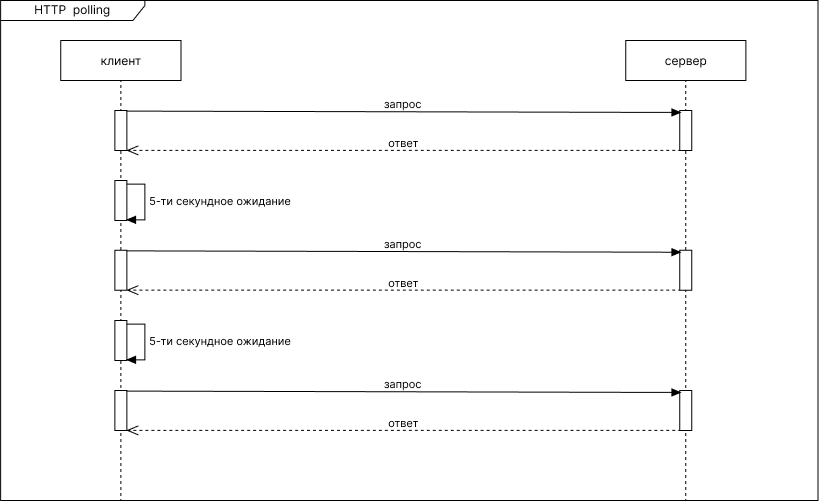
\includegraphics[width=1.0\hsize]{fig/http-polling.png}\\[2mm]
\caption{HTTP polling}\label{fig:http-polling}
\end{center}
\end{figure}

Основные недостатки метода HTTP polling:

\begin{enumerate} 
  \item Обновление состояние будет иметь задержку в тот промежуток времени, через который выполняются запросы.
  
  \item Большую часть времени сервер будет возвращать пустые запросы, из-за чего интернет-трафик будет расходоваться в пустую.
\end{enumerate}

\subsection{Использование HTTP long polling для обновления состояния приложения}

HTTP long polling — механизм, при котором клиент делает HTTP запрос и ожидает ответа от сервера, cсервер вернет ответ тогда, когда запрашиваемый ресурс будет доступен. HTTP соединение остается открытым до тех пор, пока запрашиваемый ресурс не станет доступен или не истечет время ожидания запроса. Когда ответ получен, соединение закрывается, клиент делает новые запрос, и цикл продолжается \cite{HttpLongPolling}. Выполнение HTTP long polling продемонстрировано в виде диаграммы последовательности на рисунке \ref{fig:http-longpolling}. 

\begin{figure}[H]
\begin{center}
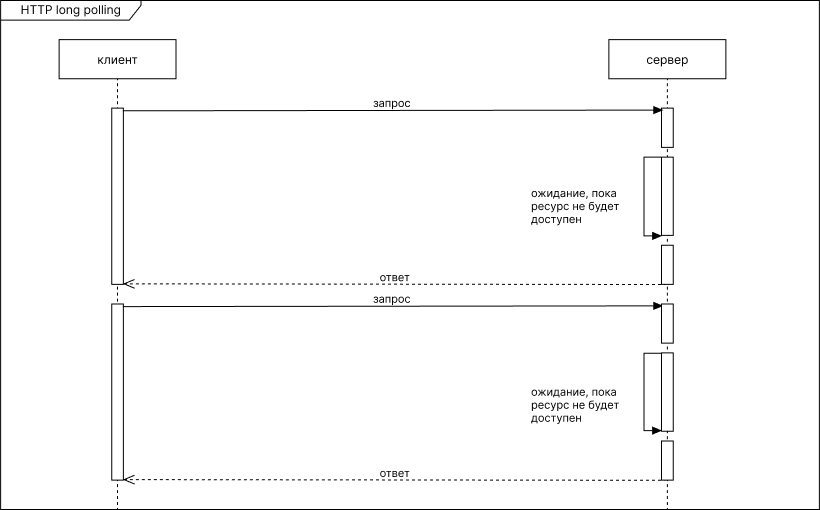
\includegraphics[width=1.0\hsize]{fig/http-longpolling.png}\\[2mm]
\caption{HTTP long polling}\label{fig:http-longpolling}
\end{center}
\end{figure}

Основным недостатком данного метода является то, что в большинстве случаев запрос будет обрываться из-за превышения времени ожидания, после чего клиент должен будет затратить ресурсы на установление нового подключения к серверу.

Более простым решением было бы использование одного TCP соединения для обмена сообщениями в обоих направлениях, этот функционал обеспечивается альтернативой HTTP polling — WebSocket, который будет рассмотрен далее.

\section{Использование WebSocket для двустороннней интерактивной связи между браузером и сервером}

WebSocket — сетевое протокол на основе TCP-соединения, предназначенный для обмена сообщениями между браузером и сервером, используя постоянное полнодуплексное соединение \cite{RealTimeWebAppWsNodejs}.

Протокол WebSocket разрабатывался для замены существующих методов обмена сообщениями в реальном времени, которые используют HTTP в качестве транспортного уровня.

\subsection{Определение URI схем WebSocket}

Спецификация WebSocket определяет использование двух схем URI, используя синтаксис и терминологию спецификации URI. Схема «ws-URI» определяет незашифрованное соединение: «ws:» «//» host [ «:» port ] path [ «?» query ], «wss-URI» определяет зашифрованное соединение: «wss:» «//» host [ «:» port ] path [ «?» query ].

\subsection{Открытие WebSocket соединения}

Открытие WebSocket соединения между клиентом и сервером называется «рукопожатие», после установления соединения, канал остается открытым, и каждая сторона, независимо от другой может отправлять данные по своему желанию.

Начальное рукопожатие предназначено для обеспечения обратной совместимости с серверами на основе HTTP, чтобы один и тот же порт мог использоваться и для HTTP и для WebSocket клиентов. С этой целью, клиентский запрос на рукопожатие представляет собой HTTP запрос на обновление (листинг \ref{ls:ws-handshake}).

\begin{lstlisting}[caption={HTTP запрос на открытие WebSocket соединение}, label={ls:ws-handshake}]
GET /chatService HTTP/1.1
Host: server.example.com
Upgrade: websocket
Connection: Upgrade
Sec-WebSocket-Key: dGhlIHNhbXBsZSBub25jZQ==
Sec-WebSocket-Origin: http://example.com
Sec-WebSocket-Protocol: chat, superchat
Sec-WebSocket-Version: 13
\end{lstlisting}

Чтобы доказать клиенту, что рукопожатие было получено, сервер берет ключ, отправленный клиентом из заголовка Sec-WebSocket-Key, конкатенирует его с глобальным идентификатором имени ресурса, от результата берется хэш SHA-1, полученное значение кодируется в base64, это значение записывается в заголовок Sec-WebSocket-Accept, отправляемый сервером. Также сервер отправляет выбранный протокол из набора, предоставленного клиентом, по которому будет вестись обмен сообщениями (листинг \ref{ls:ws-handshake-response}).

\begin{lstlisting}[caption={HTTP ответ на открытие WebSocket соединение}, label={ls:ws-handshake-response}]
HTTP/1.1 101 Switching Protocols
Upgrade: WebSocket
Connection: Upgrade
Sec-WebSocket-Accept: s3pPLMBiTxaQ9kYGzzhZRbK+xOo=
Sec-WebSocket-Protocol: superchat
\end{lstlisting}

\subsection{Передача данных по протоколу WebSocket}

В протоколе WebSocket данные передаются с использованием последовательности кадров, клиент накладывает маску на все кадры, которые отправляет на сервер. Кадры WebSocket не обязательно соответствуют кадрам сетевого уровня, поскольку фрагментированное сообщение может быть объединено или разделено посредником. Кадр может содержать текстовые данные, двоичные данные, быть управляющим (для сигнализации на уровне протокола) \cite{rfc6455}. Структура кадра WebSocket показана на рисунке \ref{fig:ws-frame-format}.

\begin{figure}[H]
\begin{center}
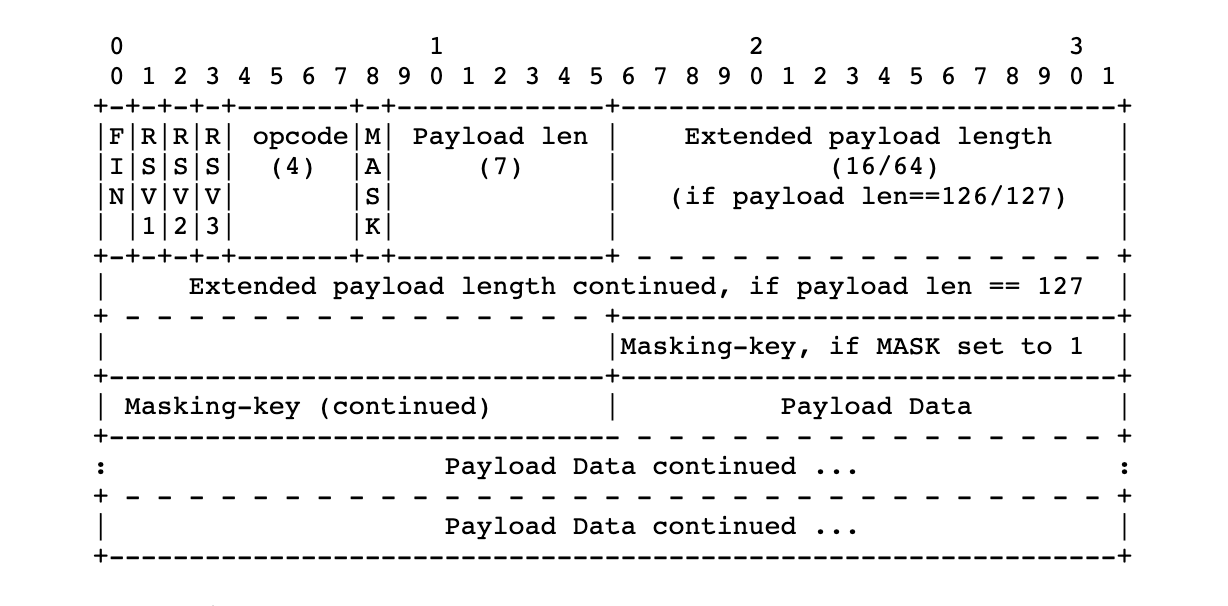
\includegraphics[width=1.0\hsize]{fig/ws-frame-format.png}\\[2mm]
\caption{Структура кадра WebSocket}\label{fig:ws-frame-format}
\end{center}
\end{figure}

\begin{enumerate} 
  \item FIN (1 bit) — указывает, что кадр является последним в сообщении.
  
  \item RSV1, RSV2, RSV3 (каждый 1 bit) — должны быть равны нулю, если не согласовано расширение, определяющие значение ненулевых значений.

  \item Opcode (4 bit) — определяет интерпретацию данных полезной нагрузки. Определены следующие значения: \%x0 — кадр продолжения, \%x1 — текстовая полезна нагрузка, \%x2 — бинарная полезная нагрузка, \%x3-7 — зарезервированы для не управляющих кадров, \%x8 — закрытие соединение, \%x9 — кадр ping, \%xA — кадр pong, \%xB-F — зарезервированы для управляющих кадров.

  \item MASK (1 bit) — определяет, маскируется ли полезная нагрузка кадра.

  \item Payload len (7 / 7 + 16 / 7 + 64 bits) — определяет длину полезной нагрузки.

  \item Masking-key (0 / 4 bytes) — маскирующие значение.

  \item Payload data (x + y bytes) — произвольные данные.
\end{enumerate}

\subsection{Предварительно определенные коды состояния в протоколе WebSocket}

В протоколе определены некоторые коды состояния, которые могут быть установлены в кадре.

\begin{enumerate} 
  \item 1000 — указывает, на штатное закрытие соединение.
  
  \item 1001 — указывает, что отправитель отключается.
  
  \item 1002 — указывает, что отправитель разрывает соединение из-за ошибки протокола.

  \item 1003 — указывает, что отправитель разрывает соединение, так как не может принять отправленный тип данных.

  \item 1004 — зарезервированное для использования в будущем.

  \item 1005 — зарезервированное значение.

  \item 1006 — зарезервированное значение.

  \item 1007 — указывает, что отправитель разрывает соединение, так как отправленные данные не соответствуют указанному типу.

  \item 1008 — указывает, что отправитель разрывает соединение, так как получил сообщение, наущающие его политику.

  \item 1009 — указывает, что отправитель разрывает соединение, так как отправленное сообщение слишком велико для обработки.

  \item 1010 — указывает, что отправитель разрывает соединение, так как ожидал, что сервер согласует одно или несколько расширений, но не получил его в ответном рукопожатии.

  \item 1011 — указывает, что отправитель разрывает соединение, так как возникла непредвиденная ситуация.

  \item 0-999 — не используются.

  \item 1000-2999 — зарезервированы для использования протоколом, его будущими версиями и расширениями.

  \item 3000-3999 — зарезервированы для использования библиотеками, платформами и приложениями. Кода состояния должны быть зарегистрированы в IANA.

  \item 3000-3999 — зарезервированы для частного использования. Могут использовать по предварительному соглашению между приложениями.
\end{enumerate}

\section{Использование WebRTC для организации передачи потоковых данных}

WebRTC (Web Real Time Communications) — набор протоколов, описывающих передачу потоковых данных между браузерами в реальном времени, а также между браузерами и другими субъектами \cite{WebRTCStandardization}.

WebRTC является оркестратором, объединяя множество существующих специализированных технологий в единое целое, позволяя изучать каждую из них по-отдельности. Технологии входящие в WebRTC показаны на рисунке \ref{fig:webrtc}. 

\begin{figure}[H]
\begin{center}
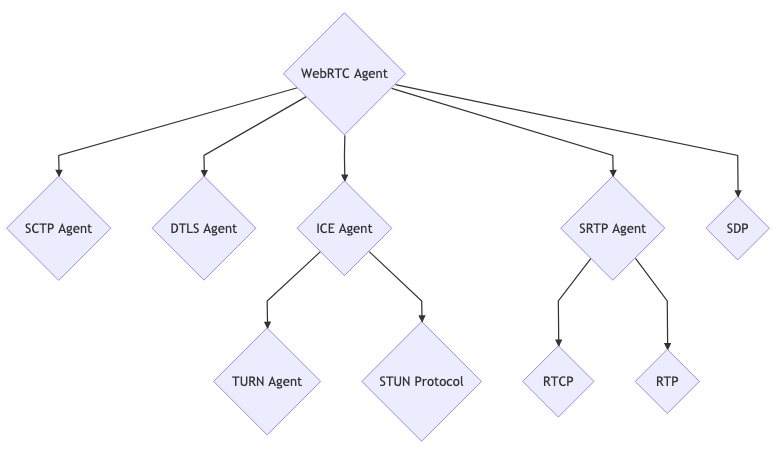
\includegraphics[width=1.0\hsize]{fig/webrtc.png}\\[2mm]
\caption{Технологии входящие в WebRTC}\label{fig:webrtc}
\end{center}
\end{figure}

При запуске WebRTC клиент не знает того, с кем будет происходить коммуникация, для этого, перед установкой соединение осуществляется сигнализация. Сигнализация осуществляется при помощи протокола SDP (Session Description Protocol), в сигнальном сообщении определяется количество аудио и видео треков, какие аудио и видео кодеки поддерживаются каждым субъектом, значения, используемые для обеспечения безопасности, значения, используемые в процессе подключения. Сигнализация проходит вне WebRTC, для этого используют HTTP запросы или WebSocket соединение \cite{rfc8835}.

Для установления подключения используется протокол ICE (Interactive Connectivity Establishment) — позволяет установить соединение между двумя субъектами.

Обеспечение безопасности при использовании WebRTC достигается за счет использования двух протоколов — DLTS (Datagram Transport Layer Securit) и SRTP (Secure Real-time Transport Protocol).

DLTS является просто TLS (криптографических протокол, для безопасной коммуникации через HTTPS) наложенным поверх UDP. Сначала выполняется рукопожатие DLTS. WebRTC проверяет, что сертификат, переданный через DTLS, совпадает с отпечатком, переданным в процессе сигнализации. После процесса рукопожатия, DLTS соединение используется для передачи сообщений.

SRTP используется для зашифрованной передачи аудио и видео потоков. Сессия SRTP начинается с извлечения ключей из установленной DTLS сессии.

После установки безопасного двунаправленного соединение между двумя субъектами, можно приступить к обмену информацией. WebRTC определяет два протокола коммуникации между пирами: SCTP и RTP. SCTP (Stream Control Transmission Protocol) — используется для отправки и приема сообщений, зашифрованных с помощью DTLS. По нему определяется множество настроек связанных с доставкой сообщений. RTP (Real-time Transport Protocol) — используется для передачи медиа потоков, зашифрованных с помощью SRTP \cite{WebRTCSCTP}.

\section{Перспективы развития методов и средсв коммуникации в режиме реального времени}

На данный момент, в разработке современных веб-приложений принято использовать WebSocket для двухстороннего обмена текстовыми сообщениями между клиентом и сервером с гарантией доставки через TCP соединение. При использовании TLS шифрования, для открытия TCP соединения требуется пройти несколько циклов отправки-приема пакетов, что вызывает значительные задержки \cite{WebRTCCongestion}.

С 2012 года, компания Google начала разработку протокола для замены устоявшегося стека TCP+TLS+HTTP/2, поскольку TCP реализован в ядрах операционных систем и его изменение практически невозможно, новый протокол был построен на базе UDP, который не имеет каких-либо серьезных ограничений.

QUIC (Quick UDP Internet Connections) — безопасный транспортный протокол общего назначения. Основные особенности в том, что протокол QUIC является безопасным по умолчанию, сокращает время соединение до 0 циклов в общем случае, реализует мультиплексирование без блокировки начала очереди, использует сжатие заголовков QPACK \cite{rfc9000}.

В мае 2021 года IETF официально опубликовало QUIC как RFC 9000. Начиная с Chrome 93, поддержка RFC 9000 включена по умолчанию для всех пользователей. В июне 2022 года IETF выпустила стандартизацию протокола HTTP/3, опубликованный как RFC 9114. Новый протокол предназначен для решения некоторых проблем HTTP/2, а именно улучшение взаимодействия с пользователем, уменьшение влияния потери пакетов без блокировки начала очереди, ускорение рукопожатия, включение шифрования по умолчанию \cite{rfc9114}.

Основной особенностью HTTP/3 является использования протокола QUIC на транспортном уровне, а сам HTTP/3 является относительно небольшой адаптацией HTTP/2, чтобы сделать его совместимым с новым транспортным протоколом. Сравнение стеков TCP+TLS+HTTP/2 и UDP+QUIC+HTTP/3 показано на рисунке \ref{fig:protocol-stack}.

\begin{figure}[H]
\begin{center}
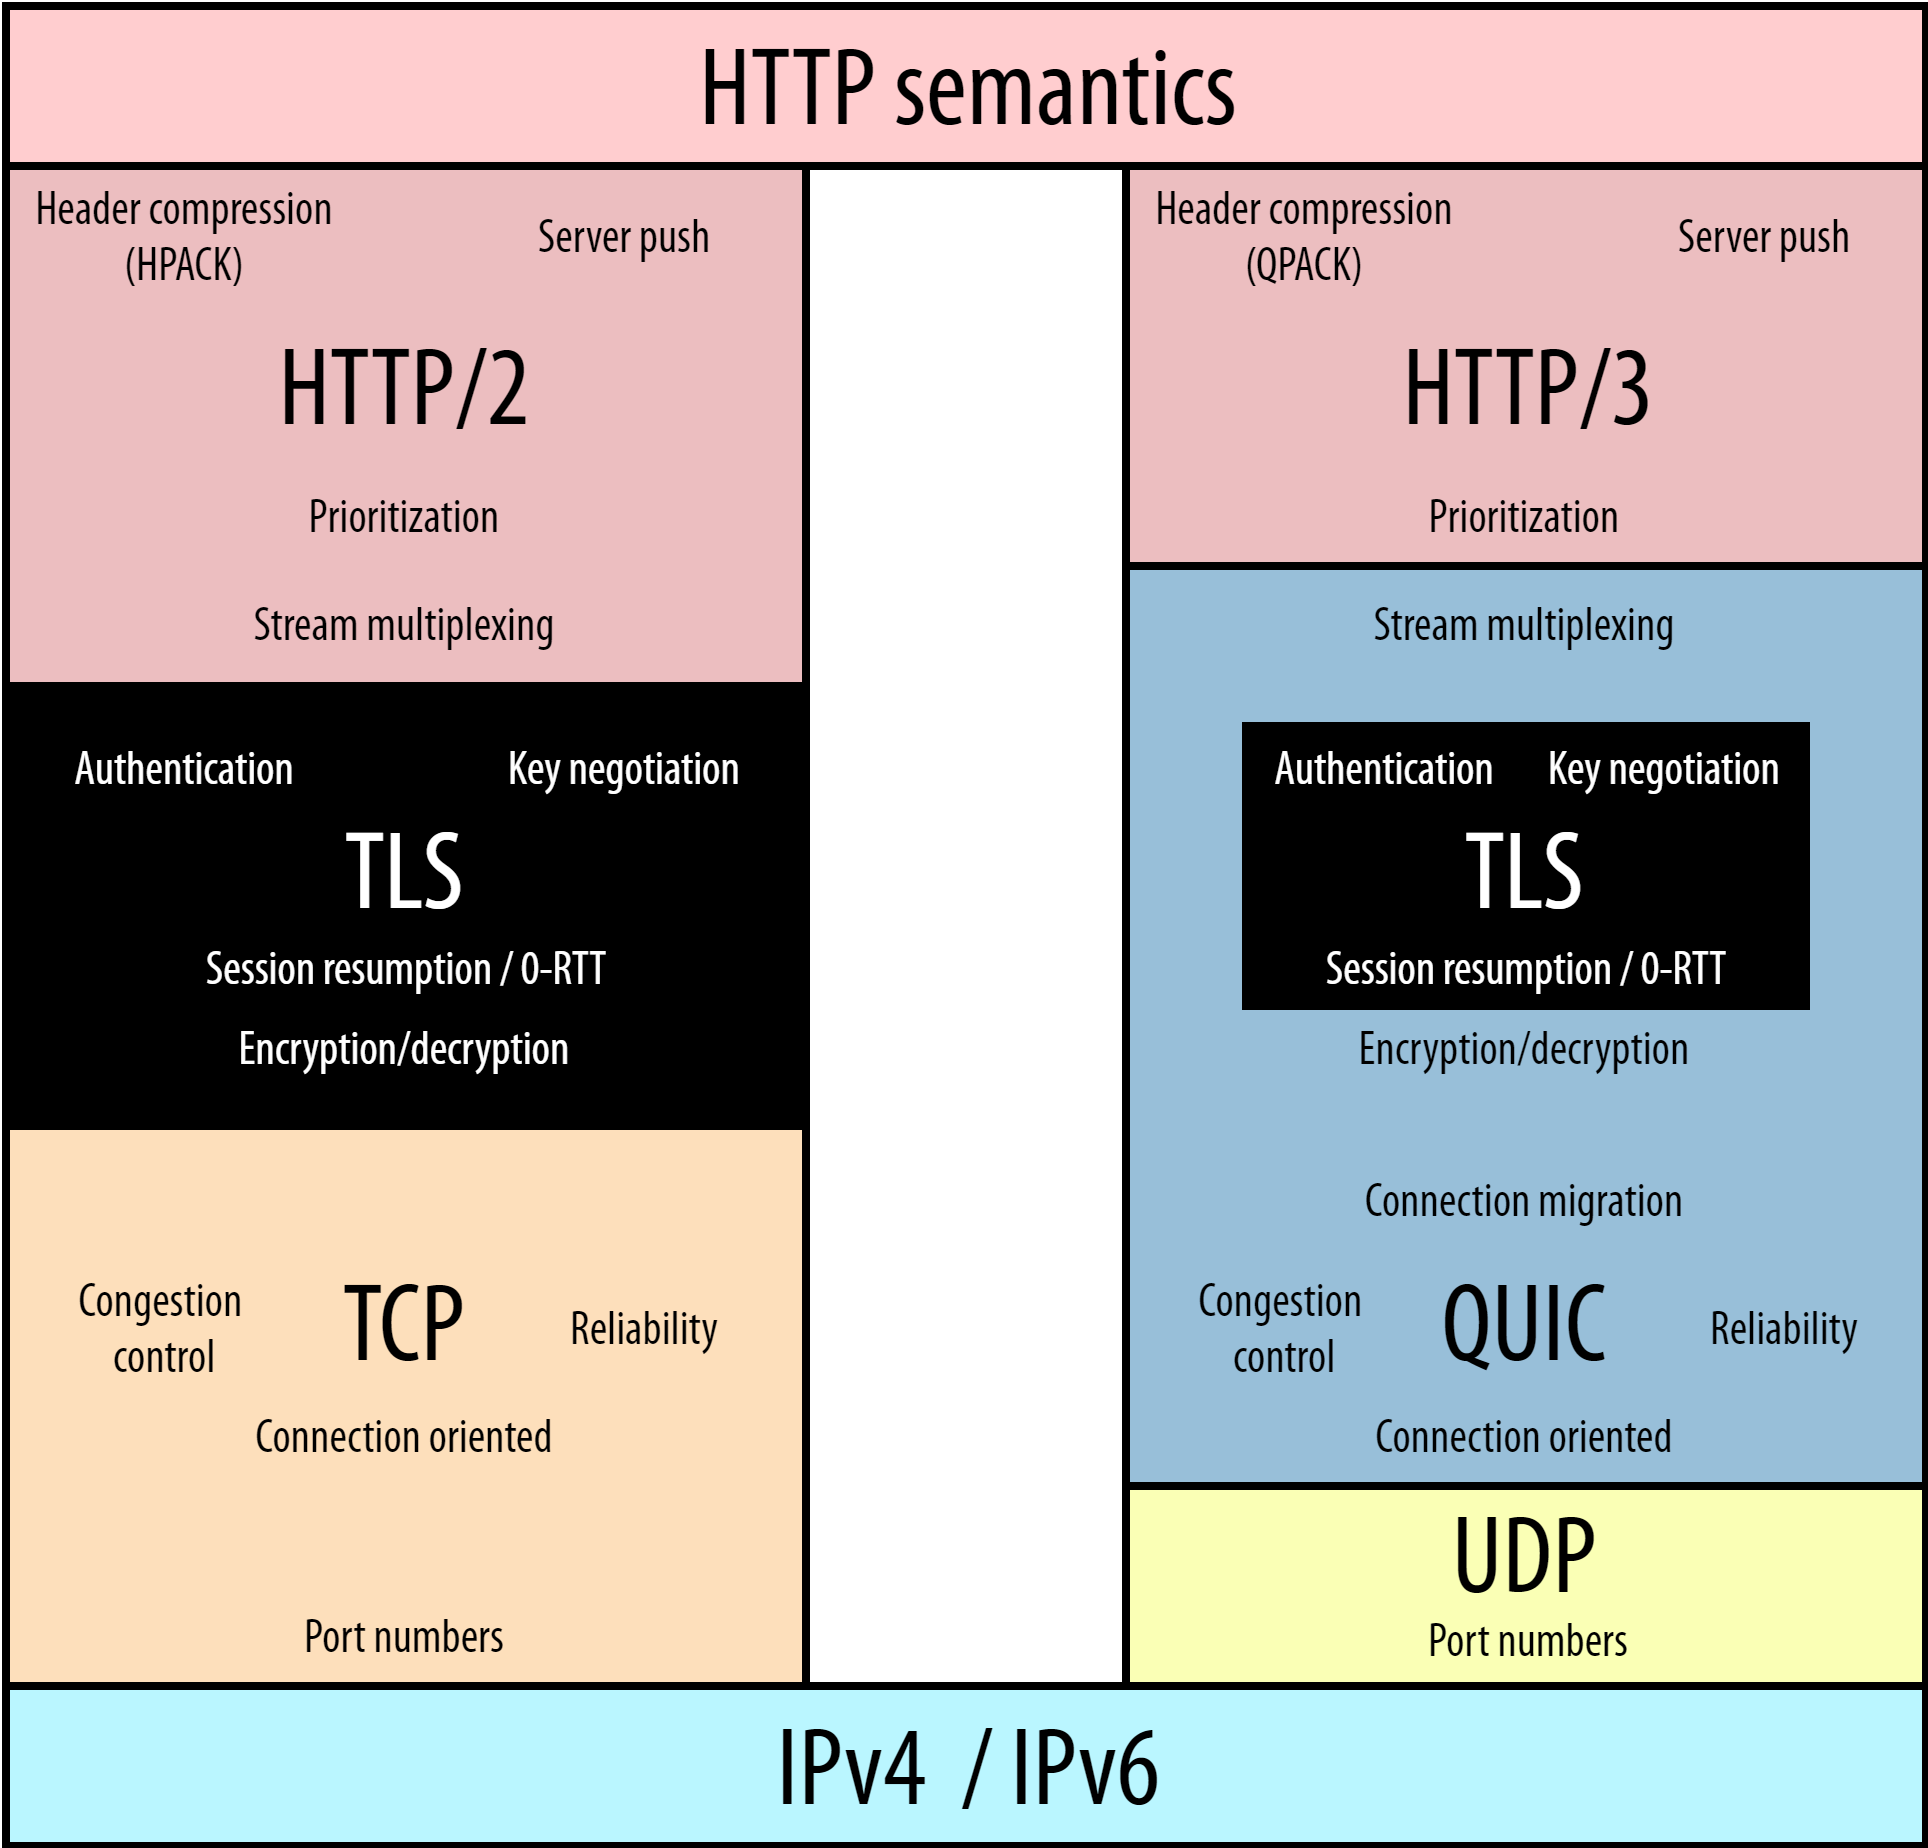
\includegraphics[width=1.0\hsize]{fig/protocol-stack.png}\\[2mm]
\caption{Сравнение стека TCP+TLS+HTTP/2 и UDP+QUIC+HTTP/3}\label{fig:protocol-stack}
\end{center}
\end{figure}

С постепенным внедрением QUIC в браузеры, W3C была опубликована черновая спецификация «WebTransport», определяющая набор ECMAScript APIs, предлагающих двунаправленный обмен сообщениями между клиентом и сервером с малой задержкой \cite{WebTransport}. Данный API в будущем может заменить WebSocket и WebRTC.

WebTransport использует протокол HTTP/3 для двунаправленной коммуникации. Интерфейс поддерживает отправку данных через дейтаграммы и потоки.

Дейтаграммы подходят для отправки и получения данных, для которых не требуются строгие гарантии доставки. Потоки обеспечивают надежную упорядоченную передачу данных, использование нескольких потоков аналогично использованию нескольких TCP соединений, но благодаря использованию QUIC, их открытие и закрытие не влечет больших затрат.

WebTransport поддерживает только соединение клиент-сервер, в отличии от WebRTC, который имеет поддержку одноранговой связи. Исходя из этого, WebTransport не будет альтернативой WebRTC в случае, если необходимо общение между несколькими клиентами \cite{WebTransportW3C}.

На текущий момент проводятся испытания технологии и доработка спецификации, WebTransport был реализован в Chrome 97, также ожидается внедрение в остальные браузеры.